\section{Main Processor} \label{sec:MCU}

This section outlines the behavior of the main processor, or MCU. The MCU processes sampled voltage and current waveforms and configures the Sample Control Module with parameters like sample size, sample frequency, and test frequency. Although the original plan was for the Sample Control Module to manage tasks such as auto-ranging, adjusting PGA gain, and setting the test-signal level, these have been incorporated into the MCU's responsibilities due to time constraints. Implementing such non-time-critical functions in C rather than HDL proved to be both easier and quicker.

The process for determining the impedance of a Device Under Test (DUT) involves several steps:

Initially, a small sample size, capturing just a few full waveforms of the test frequency, is set for the Sample Control Module. Sampling begins, and after completion, the MCU checks if the sampled signal is either saturated or not fully utilizing the ADC's full dynamic range. Based on this check, adjustments are made to the range resistors and PGA settings. 

Next, the sample size is adjusted in the Sample Control Module, and sampling is reinitiated. Once the new sampling is done, the MCU retrieves these samples, applies a Discrete Fourier Transform (DFT) to analyze them, and then calculates the impedance using the frequency-domain representations of voltage and current. After calculation, necessary corrections are applied to the impedance values. The final step, which was not completed by the time of this report, involves displaying this impedance through a user interface.

The key segments of the C code executed on the STM32F446RE microcontroller are detailed in this section. The full C code can be found in appendix \refq{App:MCUCode}.

The code is organized into data structures that group related functions and variables, giving greater modularity and readability. An example can be seen in code listing \refq{lst:CACODE} where all functions and variables related to analyzing an impedance can be seen.

\lstinputlisting[language=C ,style = c,firstnumber=1, linerange=277-293, caption={The code for the ComponentAnalysis datastructure.}, label={lst:CACODE}]{Appendix/Code/main_2612.tex}. 

The data structure in listing \refq{lst:CACODE} can store the impedance in rectangular form, or the admittance in polar form, in the DUT instance of the "parameters" data type inside the ComponentAnalysis structure. Various functions are required to analyze the DUT and the ones specifically for analyzing an impedance, i.e. not pure complex domain mathematical functions, have been assigned to the ComponentAnalysis data type in the form of callback functions.

The callback functions can be seen inside the "calculate" data structure and, at the time of submitting this report, the callback functions in the structure can be used to calculate the impedance, or admittance, of a DUT based on the current and voltage waveforms. The structure can be used to identify if the DUT is a capacitor, or inductor, calculate the loss tangent, get the value of inductance/capacitance or convert the impedance to match a series, or parallel, circuit. The implementation of these functions is, by themselves, not interesting to document in this section, however their purpose, and the theory behind them, was shown in chapter \refq{ch:TechnicalAnalysis}. The use of callbacks within the "calculate" structure allows for modular function calls, enabling easier testing and modification of impedance analysis methods without altering the main structure of the program.

The intent with this approach is to bring a small degree of \textit{object orientation} into the program. It is, of course, not object oriented programming as C does not support this, but it is an attempt to encapsulate all the necessary functionality for various modules inside a single data structure for that module as shown on figure \refq{fig:7_3_DataStructures1} with the FPGAControl data structure that contains all the functionality that the MCU needs to interact with the ADC and DAC modules inside the Sample Control module.

\begin{figure}[H]
    \centering
    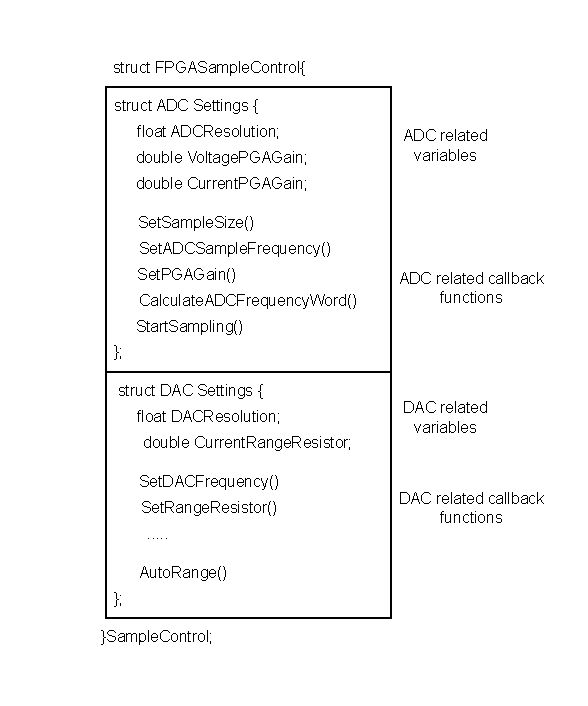
\includegraphics[clip, trim=0 25 0 25, width=0.8\textwidth]{Sections/7_SystemDesign/Figures/7_3_Datastructures FPGAControl.pdf}
    \caption{The FPGASampleControl structure has all the functions that the microcontroller needs to adjust various DAC and ADC settings. Note how not all functions for this structure is displayed on the figure.}
    \label{fig:7_3_DataStructures1}
\end{figure}

When writing the main program loop these data structures can be used to quickly identify which functions and variables are associated with a module and it gives a better overview of the C code in the project. There are several more of these data structures in this project. There are also structures that encapsulate complex number math functions, MCU to FPGA communication functions, spectral analysis functions, calibration functions and so on. All of this can be seen in appendix \refq{App:MCUCode}.